\documentclass[a4paper]{article}
\usepackage[margin=1in]{geometry}
\usepackage{graphicx}
\usepackage{enumitem}
\usepackage{listings}
\usepackage[utf8x]{inputenc}
\usepackage[spanish,es-tabla]{babel}
\usepackage{amssymb,amsmath,amsthm,amsfonts}
\usepackage{calc}
\usepackage{subcaption}
\usepackage{textcomp}
\usepackage{gensymb}
\usepackage{natbib}
\usepackage{parskip}
\usepackage{fancyhdr}
\usepackage{vmargin}
\usepackage{pdfpages}
\usepackage{pgfplots}
\usepackage{multicol}
\usepackage{multirow}
\usepackage{array}
\usepackage{booktabs}
\usepackage{wrapfig} 
\usepackage{hyperref}
\usepackage{tikz}
\usepackage{makecell}
\usepackage{float}

\usepackage[table,xcdraw]{xcolor}
\usepackage{tabularx}


\hypersetup{
    colorlinks=true,
    linkcolor=black,
    filecolor=magenta,      
    urlcolor=blue,
    }

\urlstyle{same}

\lstdefinestyle{Golang}{ % add your own preferences
    frame=single,
    basicstyle=\footnotesize,\ttfamily,breaklines=true
    keywordstyle=\color{red},
    numbers=left,
    numbersep=5pt,
    showstringspaces=false, 
    stringstyle=\color{blue},
    commentstyle=\color{green},
    tabsize=4,
    language=Go
}


\usetikzlibrary{datavisualization}
\newcolumntype{P}[1]{>{\centering\arraybackslash}p{#1}}
\newcolumntype{M}[1]{>{\centering\arraybackslash}m{#1}}

\pgfplotsset{compat=1.12}
\usepgfplotslibrary{fillbetween}
\usetikzlibrary{patterns}

% \newcommand{\gettikzxy}[3]{%
%   \tikz@scan@one@point\pgfutil@firstofone#1\relax
%   \global\edef#2{\the\pgf@x}%
%   \global\edef#3{\the\pgf@y}%
% }
% \newcommand{\gettikzcoordinates}[2]{%
%   \tikz@scan@one@point\pgfutil@firstofone#1\relax
%   \pgfmathsetmacro{\myx}{round(0.99626*\the\pgf@x/0.0283465)/1000}
%   \pgfmathsetmacro{\myy}{round(0.99626*\the\pgf@y/0.0283465)/1000}
%   \global\edef#2{(\myx,\myy)}%
% }
\makeatother

%\setmarginsrb{3 cm}{2.5 cm}{3 cm}{2.5 cm}{0.5 cm}{1 cm}{0.5 cm}{1 cm}
\title{Estudio del Flujo de control Secuencia Paralelo en Go}					                                % Titulo documento
\author{José Pinto Villamar}				                                                                              	% Autor
\date{\today}					                                                                        	% Fecha

% \makeatletter
% \let\thetitle\@title
% \let\theauthor\@author
% \let\thedate\@date
% \makeatother

\pagestyle{fancy}
\fancyhf{}
\rhead{}                                                                                        % Encabezado pagina DER
\lhead{Estudio del Flujo de control Secuencia / Paralelo en Go}                                                                        % Encabezado pagina IZQ
\cfoot{\thepage}

\newcommand{\HRule}{\rule{\linewidth}{0.5mm}}
\newcommand{\HRulee}{\rule{\linewidth}{0.2mm}}

\begin{document}
\graphicspath{{./images/}}

%%%%%%%%%%%%%%%%%%%%%%%%%%%%%%%%%%%%%%%%%%%%%%%%%%%%%%%%%%%%%%%%%%%%%%%%%%%%%%%%%%%%%%%%%
% incluir una portada de la uni en PDF
%\includepdf[pages=-, scale=1, offset=23mm -20mm]{tapa_informe.pdf}
%%%%%%%%%%%%%%%%%%%%%%%%%%%%%%%%%%%%%%%%%%%%%%%%%%%%%%%%%%%%%%%%%%%%%%%%%%%%%%%%%%%%%%%%

\begin{titlepage}
    \centering
    
    % \textsc{\LARGE Universidad La Salle}\\[0.2cm]
    \textsc{\Large Facultad de Ingenierías y Matemáticas}\\[0.2cm]
    \textsc{\Large Carrera Profesional de Ingeniería de Software}\\[0.2cm]
    \textsc{\Large Computación Distribuida y Paralela}\\[0.5cm]
    
    \centering
        \vspace*{0.0 cm}
        \begin{figure}
            \centering
            \hspace{1cm}
            
\includegraphics[height = 65px]{logo-la-salle.pdf}
            % \hspace{5cm}
            % \includegraphics[height = 100px]{dimec.png}
        \end{figure}
    
    \HRule{} \\[0.5cm]
    { \LARGE \bfseries Metodo del trapecio Secuencial/Paralelo}\\[0.3cm]
    \HRule{} \\[0.5cm]
    
    
\includegraphics[width = 0.6\textwidth]{Go_Logo_Blue.pdf}\\[0.5cm]

    \Large \emph{Docente:}\\
    Richart Smith \textsc{Escobedo Quispe}\\
    \href{mailto:r.escobedo@ulasalle.edu.pe}{r.escobedo@ulasalle.edu.pe}\\[0.5cm]
    
    \Large \emph{Desarrollado por:}\\
    José Alfredo \textsc{Pinto Villamar}\\
    \href{mailto:jpintov@ulasalle.edu.pe}{jpintov@ulasalle.edu.pe}\\[0.5cm]
    
    {\large \today}\\[2cm]
    
    \end{titlepage}
%%%%%%%%%%%%%%%%%%%%%%%%%%%%%%%%%%%%%%%%%%%

% \tableofcontents
% \pagebreak

% \listoffigures
% \listoftables
% \pagebreak

%============================================


\section{Introducción}

Como se vio en la \href{https://github.com/pintovillamar/computacion-distribuida-y-paralela/blob/main/tarea01-golang/build/report.pdf}{tarea anterior}
el lenguaje Go es un lenguaje de programación concurrente, esto quiere decir que es capaz de ejecutar varias tareas al mismo tiempo,
en este caso se va a estudiar el flujo de control secuencial y paralelo en Go.

\section{Ejecuciones en Sequencial}

\subsection{Código en Go}
%% import code from a folder
\begin{lstlisting}[style=Golang]
    package main

    import (
        "fmt"
        "math"
        "time"
    )
\end{lstlisting}
Aquí simplemente se importan las librerías necesarias para el desarrollo del código.


\begin{lstlisting}[style=Golang, firstnumber=9]
    func TrapezoidRule(f func(float64) float64, a, b float64, n int) float64 {
        h := (b - a) / float64(n)
        sum := 0.5 * (f(a) + f(b))
        for i := 1; i < n; i++ {
            sum += f(a + float64(i)*h)
        }
        return sum * h
    }
\end{lstlisting}
En esta parte del código se declara la función \texttt{TrapezoidRule}, esta función recibe como parámetros una función, un valor inicial, un valor final y un número de iteraciones.
\\

\begin{lstlisting}[style=Golang, firstnumber=18]
    func main() {

        f := func(x float64) float64 {
            return ((math.Pow(x, 2) + 1) / 2)
        }

        n := 1000

        start := time.Now()
        fmt.Println(TrapezoidRule(f, 5, 20, n))
        elapsed := time.Since(start).Nanoseconds()
        fmt.Println(elapsed)
    }
\end{lstlisting}
Es aquí donde invoco a la función \texttt{TrapezoidRule} y le paso como parámetros la función que se van a ejecutar, el valor inicial, el valor final y el número de iteraciones.
También se calcula el tiempo que tarda en ejecutarse la función.

\section{Paralelo}
\subsection{Código en Go}

\begin{lstlisting}[style=Golang]
    package main

    import (
        "fmt"
        "math"
        "time"
    )
\end{lstlisting}
En la siguiente parte del código se importan las librerías necesarias para el desarrollo del código.


\begin{lstlisting}[style=Golang,firstnumber=9]
    func worker(jobs chan int, results chan float64) {
        f := func(x float64) float64 {
            return ((math.Pow(x, 2) + 1) / 2)
        }
    
        for n := range jobs {
            results <- TrapezoidRule(f, 5, 20, n)
        }
    }
\end{lstlisting}
En la siguiente función \texttt{worker} se crea un canal de entrada y otro de salida, en este caso el canal de entrada es \texttt{jobs} y el canal de salida es \texttt{results}.
Aquí se llama a la función $f(x) = \frac{x^2+1}{2}$ y se le asigna el valor de $n$ que se recibe por el canal de entrada. Y se envía el resultado por el canal de salida.
\\

\begin{lstlisting}[style=Golang,firstnumber=19]
    func TrapezoidRule(f func(float64) float64, a, b float64, n int) float64 {
        h := (b - a) / float64(n)
        sum := 0.5 * (f(a) + f(b))
        for i := 1; i < n; i++ {
            sum += f(a + float64(i)*h)
        }
        return sum * h
    }

\end{lstlisting}
En esta parte se declara la función \texttt{TrapezoidRule}, esta función recibe como parámetros una función, un valor inicial, un valor final y un número de iteraciones.
\\

\begin{lstlisting}[style=Golang,firstnumber=28]
    func main() {

        n := 1000
    
        jobs := make(chan int, n)
        results := make(chan float64, n)
    
        go worker(jobs, results)
        go worker(jobs, results)
    
        start := time.Now()
        for i := 0; i < n; i++ {
            jobs <- i
        }
        elapsed := time.Since(start).Seconds()
        fmt.Println(elapsed)
    
        close(jobs)
    
        // for i := 0; i < n; i++ {
        // 	fmt.Println(<-results)
        // }
    }
  
\end{lstlisting}
Y como parte final, se crea la clase main donde se asignan workers, se envían los valores de $n$ por el canal de entrada y se recibe el resultado por el canal de salida.
También se declara el numero de iteraciones y los resultados que saldrán por los canales.
También se calcula el tiempo en que se tardan en ejecutar cada una de las funciones.
Inclusive se puede crear más workers para que el trabajo sea más rápido/eficiente.
Al final se cierra \texttt{jobs} y si se desea se pueden imprimir los resultados.
\\

\section{Resultados}
% Please add the following required packages to your document preamble:
% \usepackage[table,xcdraw]{xcolor}
% If you use beamer only pass "xcolor=table" option, i.e. \documentclass[xcolor=table]{beamer}
Las siguientes gráficas son muestra de las pruebas que se hicieron.
Se realizó 10 pruebas en cada ciclo, es decir, en 1 trapecio, se realizaron
10 pruebas para sacar el promedio de tiempo. Y así sucesivamente. \\
\begin{figure}[H]
\centering
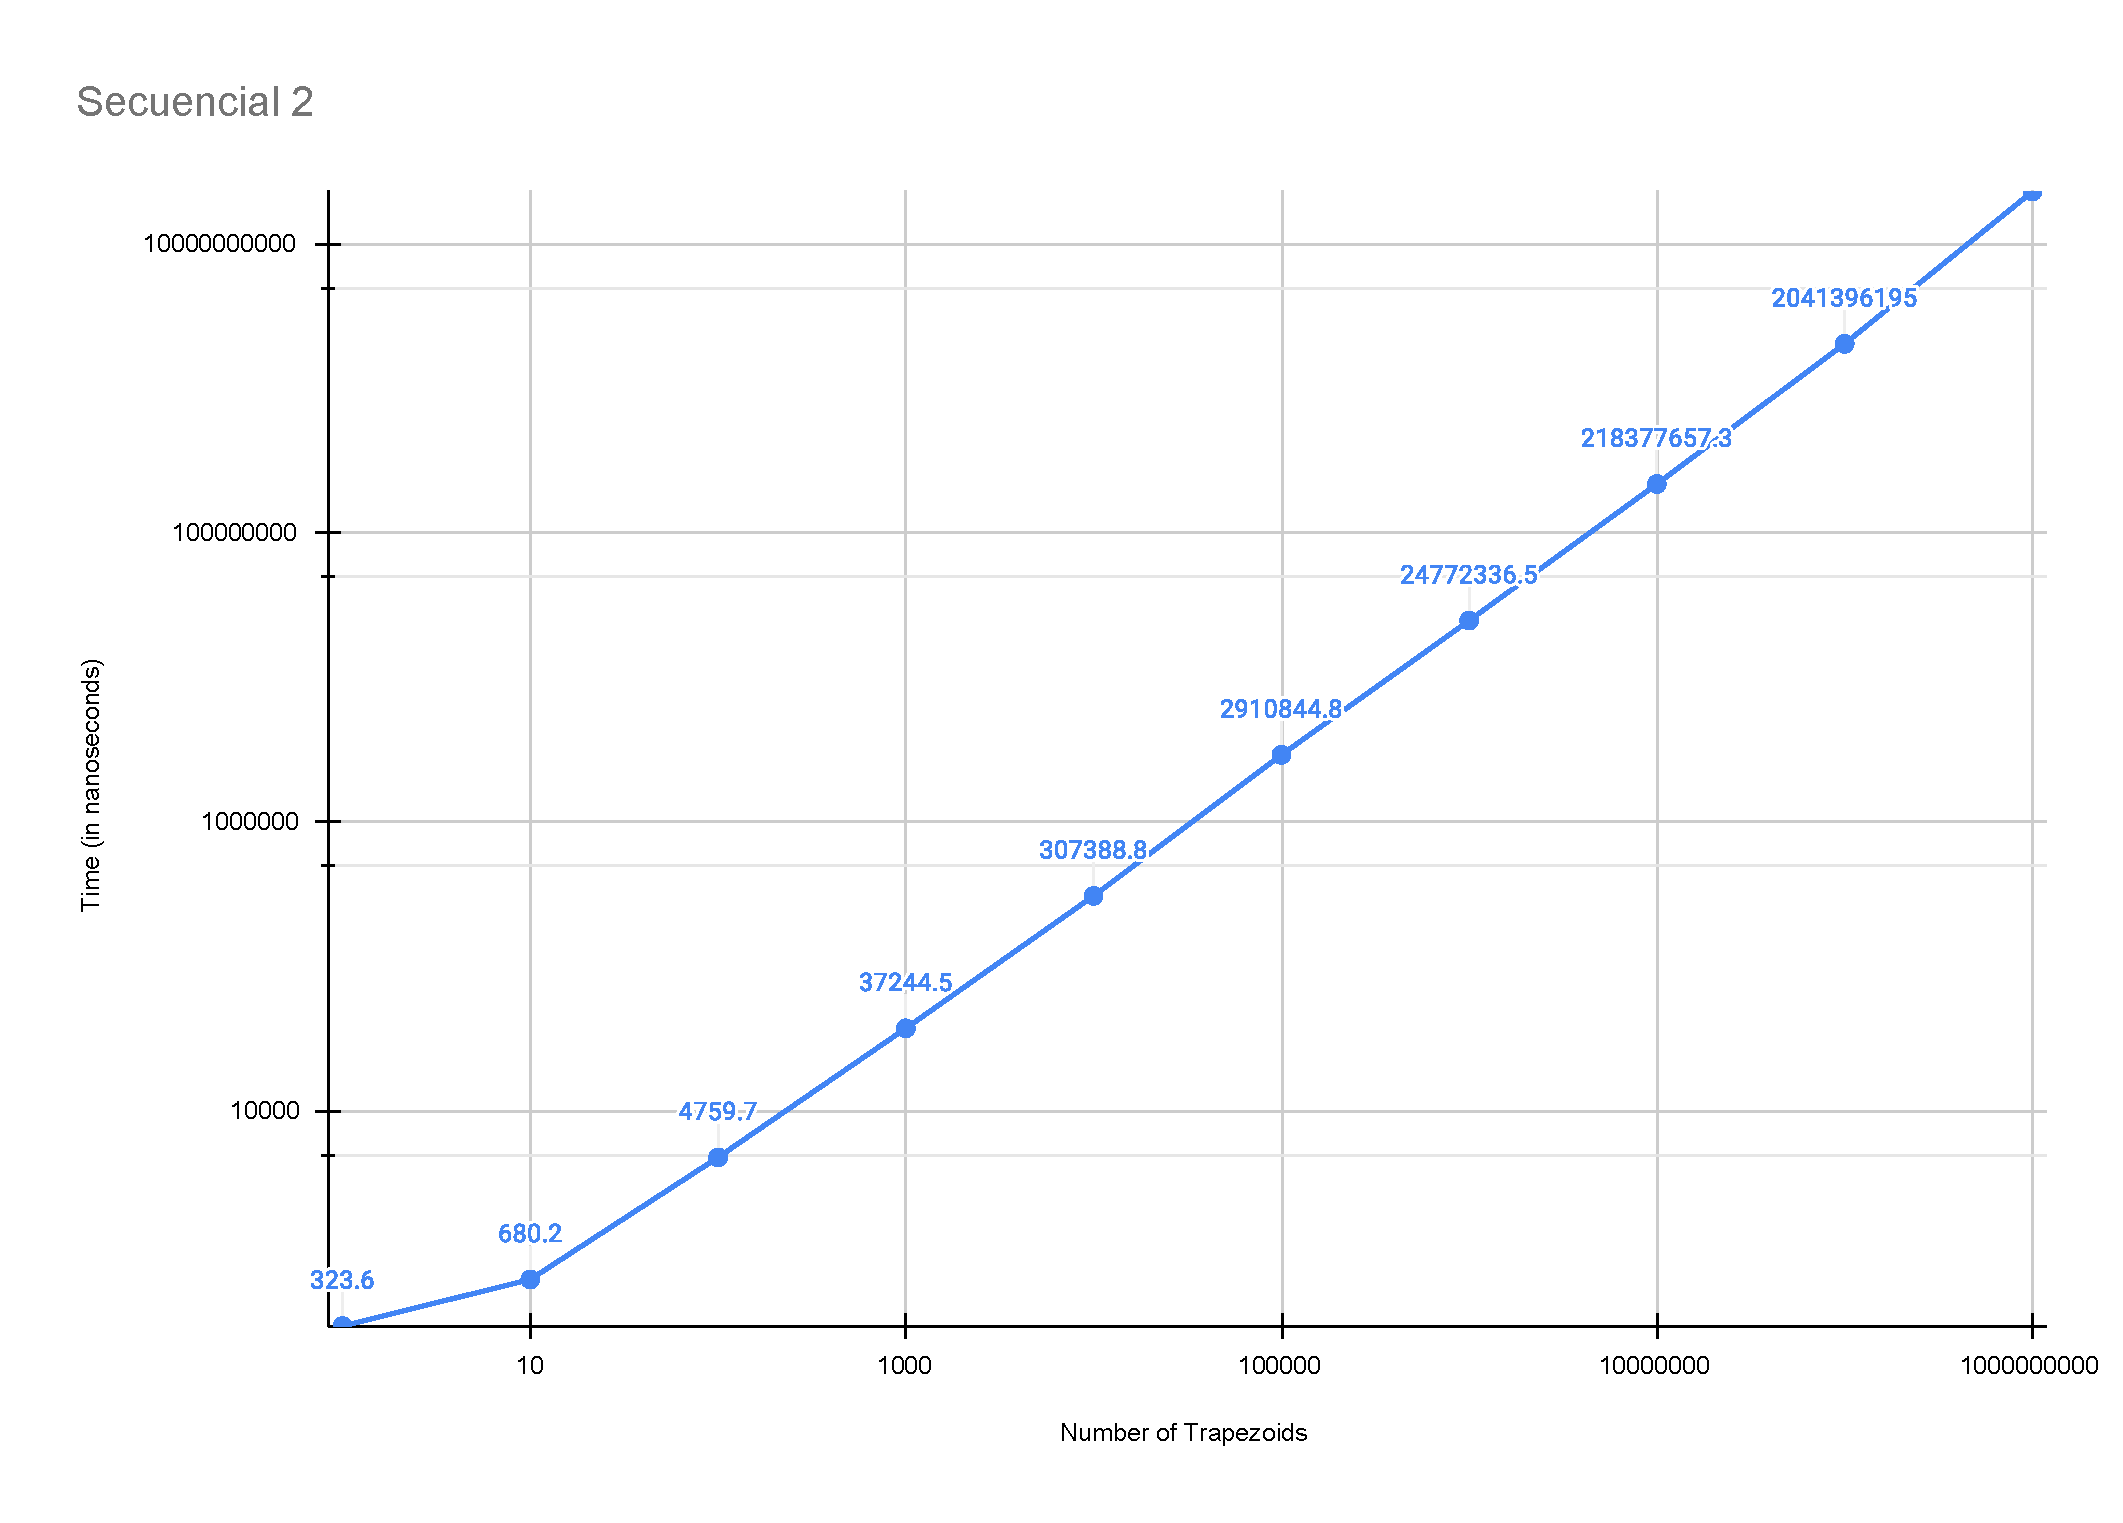
\includegraphics[width=\textwidth]{Secuencial 2.pdf}
\caption{Tiempo de ejecución de la regla del trapecio en programación secuencial.}
\end{figure}

\begin{figure}[H]
\centering
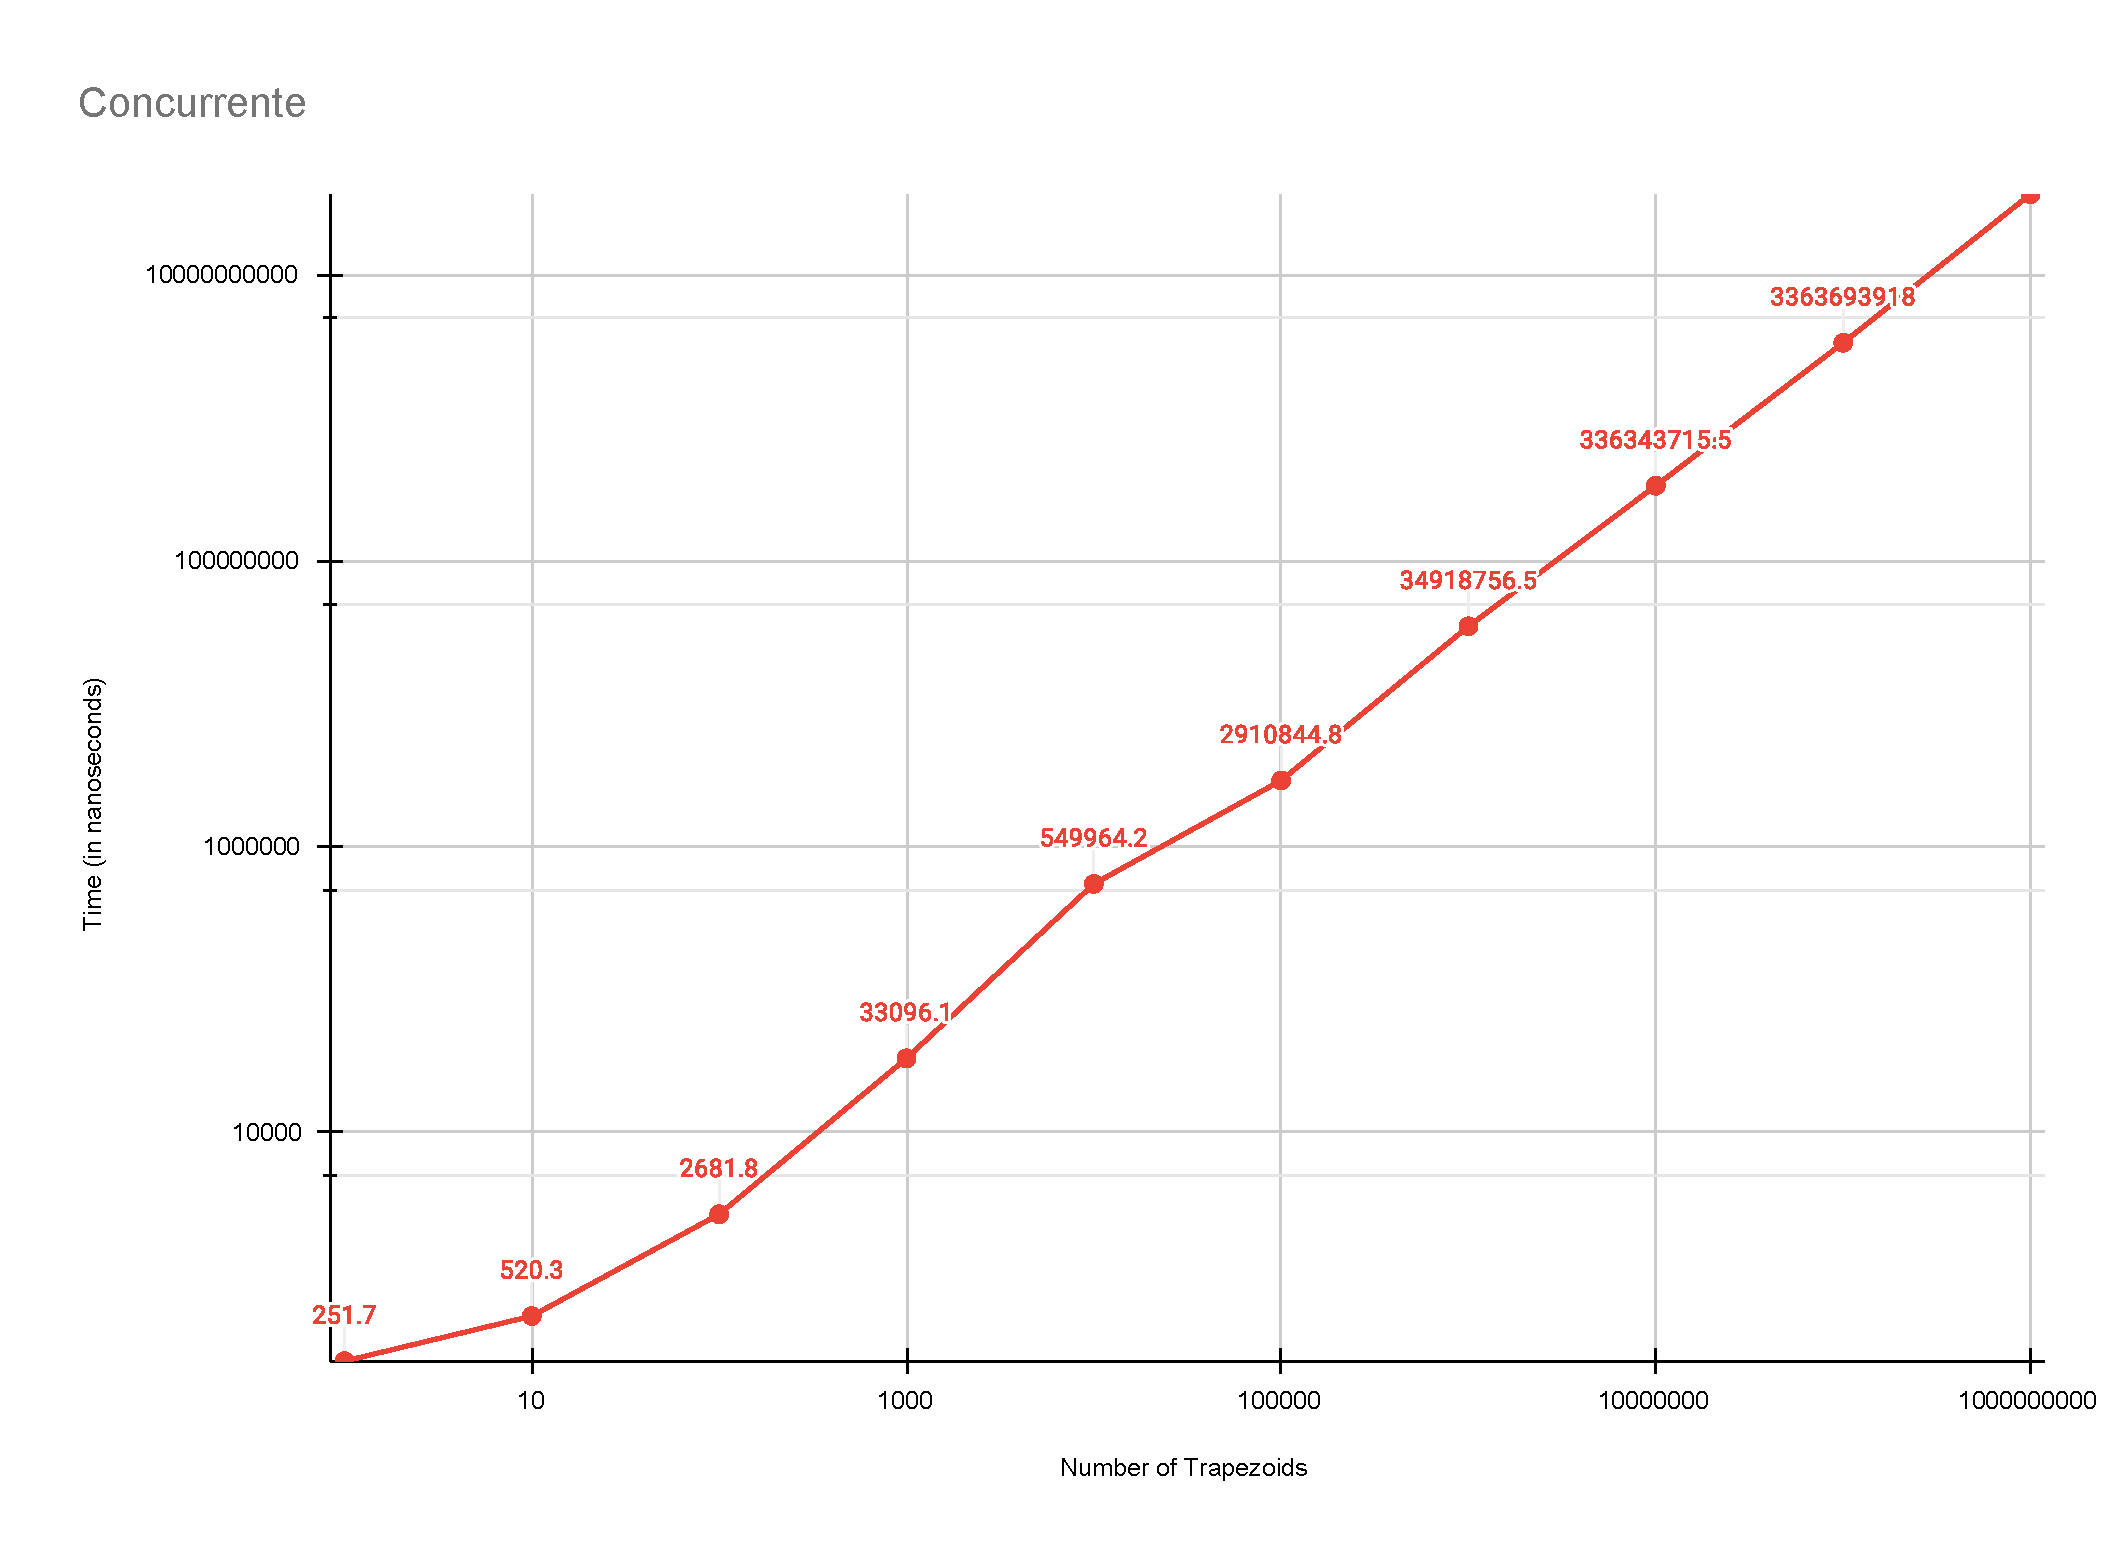
\includegraphics[width=\textwidth]{Concurrente.pdf}
\caption{Tiempo de ejecución de la regla del trapecio en programación concurrente.}
\end{figure}

\begin{figure}[H]
\centering
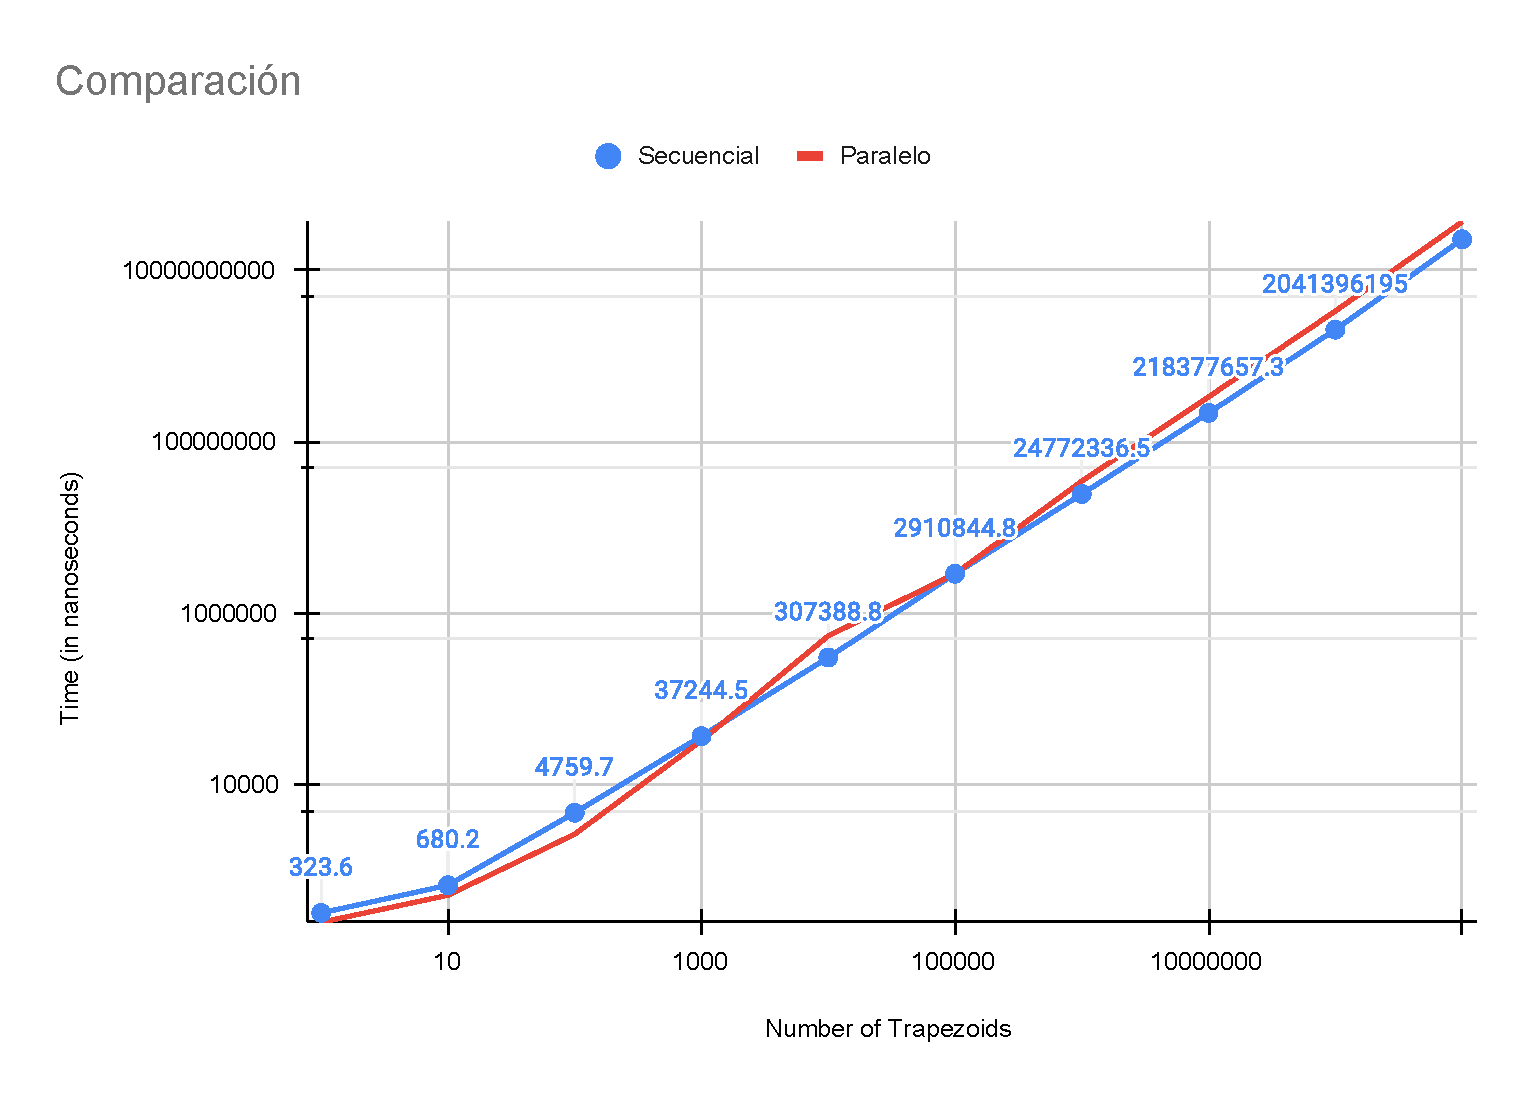
\includegraphics[width=\textwidth]{Comparacion.pdf}
\caption{Comparación entre la programación secuencial y concurrente.}
\end{figure}


\section{Repositorio}
\begin{itemize}
\item \href{https://github.com/pintovillamar/computacion-distribuida-y-paralela/tree/main/tarea02-golang}{https://github.com/pintovillamar/computacion-distribuida-y-paralela/tree/main/tarea02-golang}
\end{itemize}


\bibliographystyle{ieeetr}
\bibliography{refs.bib}


\end{document}